\chapter{Transformada de Laplace}

\section{Definición y condiciones de existencia}

\begin{definition}
Sea $f(t)$ una función definida para $t \ge 0$. Su \textbf{transformada de Laplace} se define como la integral impropia
\[
\mathcal{L}\{f(t)\} = \int_0^\infty e^{-st} f(t)\,dt,
\]
siempre que esta integral impropia converja para algún valor de $s$ (los criterios de convergencia de integrales impropias del Capítulo~\ref{cap:impropias} son la herramienta de fondo). El resultado, denotado por $F(s)$ o $\mathcal{L}\{f\}$, es una función de la variable compleja $s$ (aunque en la práctica suele considerarse $s$ real y $s>a$ para cierta constante $a$).
\end{definition}

\begin{rem}
La transformada de Laplace es una herramienta muy útil para resolver ecuaciones diferenciales lineales con coeficientes constantes, ya que transforma derivadas en operaciones algebraicas y convierte condiciones iniciales en términos sencillos. Además, maneja de forma natural funciones discontinuas o impulsivas.
\end{rem}

\begin{definition}[Orden exponencial]
Se dice que $f(t)$ es de \textbf{orden exponencial} si existen constantes $M>0$, $a\in\mathbb R$ y $T>0$ tales que
\[
|f(t)| \le M e^{a t}\quad \forall t\ge T.
\]
\end{definition}

\begin{theorem}[Condiciones suficientes de existencia]
Si $f(t)$ es continua por tramos en $[0,\infty)$ y de orden exponencial, entonces su transformada de Laplace $\mathcal{L}\{f(t)\}$ existe para todo $s>a$, donde $a$ es la constante de orden exponencial.
\end{theorem}

\begin{rem}
La continuidad por tramos permite que la función tenga un número finito de saltos en cualquier intervalo finito; esto incluye a las funciones escalón y a las funciones definidas por tramos típicas en ingeniería.
\end{rem}

A continuación se presentan las transformadas de Laplace de las funciones elementales más comunes. Todas ellas se obtienen directamente de la definición, y serán de uso constante en el resto del capítulo.

\begin{center}
\begin{tabular}{c|c}
$f(t)$ & $F(s)=\mathcal{L}\{f(t)\}$ \\ \hline
$1$ & $\dfrac{1}{s}$ \quad $(s>0)$ \\[6pt]
$e^{at}$ & $\dfrac{1}{s-a}$ \quad $(s>a)$ \\[6pt]
$\cos(bt)$ & $\dfrac{s}{s^2+b^2}$ \quad $(s>0)$ \\[6pt]
$\sen(bt)$ & $\dfrac{b}{s^2+b^2}$ \quad $(s>0)$ \\[6pt]
$t^n$ ($n=0,1,2,\dots$) & $\dfrac{n!}{s^{n+1}}$ \quad $(s>0)$
\end{tabular}
\end{center}

\begin{example}[Cálculo directo de la transformada de $f(t)=1$]
Calcular $\mathcal{L}\{1\}$ usando la definición.
\begin{myproof}
\textbf{Paso 1.} Planteamos la integral impropia:
\[
\mathcal{L}\{1\} = \int_0^\infty e^{-st}\cdot 1\,dt = \lim_{b\to\infty}\int_0^b e^{-st}\,dt.
\]

\textbf{Paso 2.} Resolvemos la integral:
\[
\int_0^b e^{-st}\,dt = \left.-\frac{1}{s}e^{-st}\right|_0^b = -\frac{1}{s}e^{-sb} + \frac{1}{s}.
\]

\textbf{Paso 3.} Tomamos el límite $b\to\infty$; para $s>0$,
\[
\lim_{b\to\infty}\left(-\frac{1}{s}e^{-sb}+\frac{1}{s}\right) = \frac{1}{s}.
\]
Por tanto,
\[
\boxed{\mathcal{L}\{1\} = \frac{1}{s},\quad s>0.}
\]
\end{myproof}
\end{example}

\begin{example}[Cálculo directo de la transformada de $f(t)=e^{at}$]
Obtener $\mathcal{L}\{e^{at}\}$ a partir de la definición.
\begin{myproof}
\textbf{Paso 1.} Escribimos la integral:
\[
\mathcal{L}\{e^{at}\} = \int_0^\infty e^{-st} e^{at}\,dt = \int_0^\infty e^{-(s-a)t}\,dt.
\]

\textbf{Paso 2.} Integramos:
\[
\int_0^b e^{-(s-a)t}\,dt = \left.-\frac{1}{s-a}e^{-(s-a)t}\right|_0^b = -\frac{e^{-(s-a)b}}{s-a} + \frac{1}{s-a}.
\]

\textbf{Paso 3.} Para que el límite cuando $b\to\infty$ exista, necesitamos $s-a>0$, es decir $s>a$. Entonces
\[
\lim_{b\to\infty}\left(-\frac{e^{-(s-a)b}}{s-a} + \frac{1}{s-a}\right) = \frac{1}{s-a}.
\]
Luego
\[
\boxed{\mathcal{L}\{e^{at}\} = \frac{1}{s-a},\quad s>a.}
\]
\end{myproof}
\end{example}

\begin{example}[Cálculo de $\mathcal{L}\{\cos(bt)\}$ mediante definición]
Determinar la transformada de Laplace de $\cos(bt)$.
\begin{myproof}
\textbf{Paso 1.} Usamos la definición:
\[
\mathcal{L}\{\cos(bt)\} = \int_0^\infty e^{-st}\cos(bt)\,dt.
\]

\textbf{Paso 2.} Integramos por partes dos veces o utilizamos la fórmula conocida:
\[
\int e^{at}\cos(bt)\,dt = \frac{e^{at}(a\cos(bt)+b\sen(bt))}{a^2+b^2}.
\]
En nuestro caso $a=-s$, luego
\[
\int_0^T e^{-st}\cos(bt)\,dt = \left[\frac{e^{-st}(-s\cos(bt)+b\sen(bt))}{s^2+b^2}\right]_0^T.
\]

\textbf{Paso 3.} Evaluamos en $T\to\infty$: como $s>0$, $e^{-sT}\to 0$; el numerador está acotado. En $t=0$, $\cos(0)=1$, $\sen(0)=0$, por lo que
\[
\lim_{T\to\infty}\left( \frac{e^{-sT}(-s\cos(bT)+b\sen(bT))}{s^2+b^2} - \frac{-s}{s^2+b^2} \right) = \frac{s}{s^2+b^2}.
\]
Así,
\[
\boxed{\mathcal{L}\{\cos(bt)\} = \frac{s}{s^2+b^2}.}
\]
\end{myproof}
\end{example}

\begin{table}[H]
\centering
\caption{Transformadas de Laplace de uso frecuente ($s>0$, y $s>a$ en las entradas con $e^{at}$). Varias de ellas se deducen desde la definición en los ejemplos de esta sección.}
\label{tab:transformadas}
\begin{tabular}{ll}
\hline
$f(t)$ & $F(s)=\mathcal{L}\{f(t)\}$ \\
\hline
$1$ & $\dfrac{1}{s}$ \\[4pt]
$t^n\ (n\in\mathbb{N})$ & $\dfrac{n!}{s^{n+1}}$ \\[4pt]
$e^{at}$ & $\dfrac{1}{s-a}$ \\[4pt]
$\sen(\omega t)$ & $\dfrac{\omega}{s^2+\omega^2}$ \\[4pt]
$\cos(\omega t)$ & $\dfrac{s}{s^2+\omega^2}$ \\[4pt]
$e^{at}\sen(\omega t)$ & $\dfrac{\omega}{(s-a)^2+\omega^2}$ \\[4pt]
$e^{at}\cos(\omega t)$ & $\dfrac{s-a}{(s-a)^2+\omega^2}$ \\[4pt]
$t^n e^{at}$ & $\dfrac{n!}{(s-a)^{n+1}}$ \\[4pt]
$u(t-a)$ & $\dfrac{e^{-as}}{s}$ \\[4pt]
$\delta(t-a)$ & $e^{-as}$ \\
\hline
\end{tabular}
\end{table}

\section{Propiedades fundamentales de la transformada}

\begin{theorem}[Linealidad]
La transformada de Laplace es lineal: para cualesquiera constantes $a,b$ y funciones $f,g$ cuyas transformadas existan,
\[
\mathcal{L}\{a f(t) + b g(t)\} = a\,\mathcal{L}\{f(t)\} + b\,\mathcal{L}\{g(t)\}.
\]
\end{theorem}

\begin{example}[Uso de linealidad]
Calcular $\mathcal{L}\{4e^{3t} - 2\cos(5t)\}$.
\begin{myproof}
\textbf{Paso 1.} Aplicamos linealidad:
\[
\mathcal{L}\{4e^{3t} - 2\cos(5t)\} = 4\mathcal{L}\{e^{3t}\} - 2\mathcal{L}\{\cos(5t)\}.
\]

\textbf{Paso 2.} Usamos la Tabla~\ref{tab:transformadas}:
\[
\mathcal{L}\{e^{3t}\} = \frac{1}{s-3},\qquad \mathcal{L}\{\cos(5t)\} = \frac{s}{s^2+25}.
\]

\textbf{Paso 3.} Sustituimos y simplificamos:
\[
4\frac{1}{s-3} - 2\frac{s}{s^2+25} = \frac{4}{s-3} - \frac{2s}{s^2+25}.
\]
Por lo tanto,
\[
\boxed{\mathcal{L}\{4e^{3t} - 2\cos(5t)\} = \frac{4}{s-3} - \frac{2s}{s^2+25}.}
\]
\end{myproof}
\end{example}

\begin{theorem}[Primer teorema de traslación (desplazamiento en $s$)]
Si $\mathcal{L}\{f(t)\}=F(s)$, entonces
\[
\mathcal{L}\{e^{at} f(t)\} = F(s-a).
\]
Es decir, multiplicar la función original por $e^{at}$ produce un desplazamiento de $a$ unidades en la variable $s$ de la transformada.
\end{theorem}

\begin{example}[Aplicación del primer teorema de traslación]
Hallar $\mathcal{L}\{e^{-2t}\sen(3t)\}$.
\begin{myproof}
\textbf{Paso 1.} Identificamos $f(t)=\sen(3t)$, luego $F(s)=\mathcal{L}\{\sen(3t)\} = \frac{3}{s^2+9}$.

\textbf{Paso 2.} El factor $e^{-2t}$ corresponde a $a=-2$. Por el primer teorema de traslación,
\[
\mathcal{L}\{e^{-2t}\sen(3t)\} = F(s-(-2)) = F(s+2).
\]

\textbf{Paso 3.} Sustituimos $s$ por $s+2$ en $F$:
\[
F(s+2) = \frac{3}{(s+2)^2+9}.
\]
Por tanto,
\[
\boxed{\mathcal{L}\{e^{-2t}\sen(3t)\} = \frac{3}{(s+2)^2+9}.}
\]
\end{myproof}
\end{example}

\begin{theorem}[Transformada de derivadas]
Sea $f(t)$ continua con derivada $f'(t)$ continua por tramos en $[0,\infty)$ y de orden exponencial. Entonces
\[
\mathcal{L}\{f'(t)\} = s F(s) - f(0),
\]
donde $F(s)=\mathcal{L}\{f(t)\}$. Más generalmente, para la derivada $n$-ésima,
\[
\mathcal{L}\{f^{(n)}(t)\} = s^n F(s) - s^{n-1}f(0) - s^{n-2}f'(0) - \cdots - f^{(n-1)}(0).
\]
\end{theorem}

\begin{example}[Transformada de derivada para resolver PVI]
Si $f(t)$ satisface $f''(t)+4f(t)=0$ con $f(0)=1,\ f'(0)=0$, calcular $\mathcal{L}\{f''(t)\}$ en términos de $F(s)$.
\begin{myproof}
\textbf{Paso 1.} Aplicamos la fórmula para $n=2$:
\[
\mathcal{L}\{f''(t)\} = s^2 F(s) - s f(0) - f'(0).
\]

\textbf{Paso 2.} Sustituimos las condiciones iniciales $f(0)=1$ y $f'(0)=0$:
\[
\mathcal{L}\{f''(t)\} = s^2 F(s) - s(1) - 0 = s^2 F(s) - s.
\]

\textbf{Paso 3.} De la ecuación diferencial, $\mathcal{L}\{f''(t)\} + 4\mathcal{L}\{f(t)\}=0$, es decir
\[
s^2 F(s) - s + 4F(s)=0 \implies F(s)=\frac{s}{s^2+4}.
\]
Así,
\[
\boxed{\mathcal{L}\{f''(t)\} = s^2\left(\frac{s}{s^2+4}\right) - s = \frac{s^3}{s^2+4} - s.}
\]
\end{myproof}
\end{example}

\begin{theorem}[Transformada de integrales]
Si $F(s)=\mathcal{L}\{f(t)\}$, entonces
\[
\mathcal{L}\left\{\int_0^t f(\tau)\,d\tau\right\} = \frac{F(s)}{s}.
\]
\end{theorem}

\begin{example}[Transformada de una integral]
Calcular $\mathcal{L}\left\{\int_0^t e^{-2\tau}\cos(3\tau)\,d\tau\right\}$.
\begin{myproof}
\textbf{Paso 1.} Sea $f(t)=e^{-2t}\cos(3t)$. Su transformada es, por el primer teorema de traslación,
\[
F(s)=\mathcal{L}\{e^{-2t}\cos(3t)\} = \frac{s+2}{(s+2)^2+9}.
\]

\textbf{Paso 2.} Por el teorema de la transformada de la integral,
\[
\mathcal{L}\left\{\int_0^t f(\tau)\,d\tau\right\} = \frac{F(s)}{s} = \frac{1}{s}\cdot \frac{s+2}{(s+2)^2+9}.
\]

\textbf{Paso 3.} Simplificamos:
\[
\boxed{\mathcal{L}\left\{\int_0^t e^{-2\tau}\cos(3\tau)\,d\tau\right\} = \frac{s+2}{s[(s+2)^2+9]}.}
\]
\end{myproof}
\end{example}

\begin{theorem}[Derivada de la transformada (multiplicación por $t$)]
Si $F(s)=\mathcal{L}\{f(t)\}$, entonces
\[
\mathcal{L}\{t^n f(t)\} = (-1)^n F^{(n)}(s),\qquad n=1,2,\dots
\]
En particular, $\mathcal{L}\{t f(t)\} = -F'(s)$.
\end{theorem}

\begin{example}[Multiplicación por $t$]
Calcular $\mathcal{L}\{t \sen(2t)\}$.
\begin{myproof}
\textbf{Paso 1.} Sea $f(t)=\sen(2t)$, con $F(s)=\frac{2}{s^2+4}$.

\textbf{Paso 2.} Derivamos $F(s)$:
\[
F'(s) = 2\cdot \frac{d}{ds}(s^2+4)^{-1} = 2\cdot (-1)(s^2+4)^{-2}\cdot 2s = -\frac{4s}{(s^2+4)^2}.
\]

\textbf{Paso 3.} Por el teorema, $\mathcal{L}\{t f(t)\} = -F'(s) = \frac{4s}{(s^2+4)^2}$.
Por tanto,
\[
\boxed{\mathcal{L}\{t\sen(2t)\} = \frac{4s}{(s^2+4)^2}.}
\]
\end{myproof}
\end{example}

\begin{theorem}[División por $t$]
Si el límite $\lim_{t\to0^+} f(t)/t$ existe y es finito, entonces
\[
\mathcal{L}\left\{\frac{f(t)}{t}\right\} = \int_s^\infty F(u)\,du,
\]
siempre que la integral impropia converja.
\end{theorem}

\begin{example}[Transformada de $(\sen t)/t$]
Calcular $\mathcal{L}\left\{\frac{\sen t}{t}\right\}$.
\begin{myproof}
\textbf{Paso 1.} Sea $f(t)=\sen t$, $F(s)=\frac{1}{s^2+1}$.

\textbf{Paso 2.} Aplicamos la fórmula:
\[
\mathcal{L}\left\{\frac{\sen t}{t}\right\} = \int_s^\infty \frac{du}{u^2+1}.
\]

\textbf{Paso 3.} Calculamos la integral:
\[
\int_s^\infty \frac{du}{u^2+1} = \left[\arctan u\right]_s^\infty = \frac{\pi}{2} - \arctan s.
\]
Por lo tanto,
\[
\boxed{\mathcal{L}\left\{\frac{\sen t}{t}\right\} = \frac{\pi}{2} - \arctan s = \arctan\left(\frac{1}{s}\right),\quad s>0.}
\]
\end{myproof}
\end{example}

\section{Transformada inversa de Laplace}

\begin{definition}
Dada una función $F(s)$, se llama \textbf{transformada inversa de Laplace} de $F$ a la función $f(t)$ tal que $\mathcal{L}\{f(t)\}=F(s)$. Se denota por
\[
f(t) = \mathcal{L}^{-1}\{F(s)\}.
\]
\end{definition}

La inversa también es lineal: $\mathcal{L}^{-1}\{aF(s)+bG(s)\}=a\mathcal{L}^{-1}\{F(s)\}+b\mathcal{L}^{-1}\{G(s)\}$.

Para calcular inversas, se usan las transformadas básicas y las propiedades, pero a menudo es necesario descomponer $F(s)$ en fracciones parciales o completar cuadrados para llevarla a formas reconocibles.

\begin{example}[Fracciones parciales: raíces reales distintas]
Hallar $\mathcal{L}^{-1}\left\{\frac{3s+5}{s^2-3s+2}\right\}$.
\begin{myproof}
\textbf{Paso 1.} Factorizamos el denominador:
\[
s^2-3s+2 = (s-1)(s-2).
\]
Planteamos la descomposición:
\[
\frac{3s+5}{(s-1)(s-2)} = \frac{A}{s-1} + \frac{B}{s-2}.
\]

\textbf{Paso 2.} Multiplicamos por $(s-1)(s-2)$:
\[
3s+5 = A(s-2)+B(s-1).
\]
Para $s=1$: $3(1)+5 = A(-1) + B(0) \Rightarrow 8 = -A \Rightarrow A=-8$.
Para $s=2$: $3(2)+5 = A(0) + B(1) \Rightarrow 11 = B$.

\textbf{Paso 3.} Entonces
\[
\frac{3s+5}{(s-1)(s-2)} = \frac{-8}{s-1} + \frac{11}{s-2}.
\]
Tomando inversa:
\[
\mathcal{L}^{-1}\left\{\frac{-8}{s-1}\right\} = -8 e^{t},\qquad \mathcal{L}^{-1}\left\{\frac{11}{s-2}\right\}=11 e^{2t}.
\]
Por tanto,
\[
\boxed{\mathcal{L}^{-1}\left\{\frac{3s+5}{s^2-3s+2}\right\} = -8e^{t} + 11e^{2t}.}
\]
\end{myproof}
\end{example}

\begin{example}[Raíces repetidas]
Calcular $\mathcal{L}^{-1}\left\{\frac{2s+3}{(s-1)^2(s+2)}\right\}$.
\begin{myproof}
\textbf{Paso 1.} Descomposición con raíz repetida:
\[
\frac{2s+3}{(s-1)^2(s+2)} = \frac{A}{s-1} + \frac{B}{(s-1)^2} + \frac{C}{s+2}.
\]

\textbf{Paso 2.} Multiplicamos por $(s-1)^2(s+2)$:
\[
2s+3 = A(s-1)(s+2) + B(s+2) + C(s-1)^2.
\]
Evaluamos:
- Para $s=1$: $2(1)+3 = A(0)+B(3)+C(0) \Rightarrow 5 = 3B \Rightarrow B=5/3$.
- Para $s=-2$: $2(-2)+3 = A(0)+B(0)+C(-3)^2 \Rightarrow -1 = 9C \Rightarrow C=-1/9$.
- Para $s=0$ (por ejemplo): $3 = A(-1)(2) + B(2) + C(1) = -2A + 2(5/3) - 1/9$.
  Entonces $3 = -2A + 10/3 - 1/9 = -2A + 30/9 - 1/9 = -2A + 29/9$.
  Despejamos: $3 - 29/9 = -2A \Rightarrow 27/9 - 29/9 = -2A \Rightarrow -2/9 = -2A \Rightarrow A=1/9$.

\textbf{Paso 3.} Entonces
\[
\frac{2s+3}{(s-1)^2(s+2)} = \frac{1/9}{s-1} + \frac{5/3}{(s-1)^2} - \frac{1/9}{s+2}.
\]
Invertimos:
\[
\mathcal{L}^{-1}\left\{\frac{1/9}{s-1}\right\} = \frac{1}{9}e^{t},\quad
\mathcal{L}^{-1}\left\{\frac{5/3}{(s-1)^2}\right\} = \frac{5}{3} t e^{t},\quad
\mathcal{L}^{-1}\left\{-\frac{1/9}{s+2}\right\} = -\frac{1}{9}e^{-2t}.
\]
Por tanto,
\[
\boxed{\mathcal{L}^{-1}\left\{\frac{2s+3}{(s-1)^2(s+2)}\right\} = \frac{1}{9}e^{t} + \frac{5}{3}t e^{t} - \frac{1}{9}e^{-2t}.}
\]
\end{myproof}
\end{example}

\begin{example}[Factores cuadráticos irreducibles: completación de cuadrados]
Hallar $\mathcal{L}^{-1}\left\{\frac{s+1}{s^2+4s+13}\right\}$.
\begin{myproof}
\textbf{Paso 1.} Completamos el cuadrado en el denominador:
\[
s^2+4s+13 = (s+2)^2 + 9.
\]
Queremos escribir el numerador como $A(s+2)+B$ para usar las fórmulas del seno y coseno desplazados.

\textbf{Paso 2.} Escribimos $s+1 = A(s+2)+B$. Igualando coeficientes:
\[
s+1 = A s + (2A+B) \Rightarrow A=1,\quad 2A+B=1 \Rightarrow 2+B=1 \Rightarrow B=-1.
\]
Entonces
\[
\frac{s+1}{(s+2)^2+9} = \frac{(s+2) - 1}{(s+2)^2+9} = \frac{s+2}{(s+2)^2+9} - \frac{1}{(s+2)^2+9}.
\]

\textbf{Paso 3.} Recordamos que
\[
\mathcal{L}^{-1}\left\{\frac{s-a}{(s-a)^2+b^2}\right\} = e^{at}\cos(bt),\qquad
\mathcal{L}^{-1}\left\{\frac{b}{(s-a)^2+b^2}\right\} = e^{at}\sen(bt).
\]
Aquí $a=-2$, $b=3$. Por tanto,
\[
\mathcal{L}^{-1}\left\{\frac{s+2}{(s+2)^2+9}\right\} = e^{-2t}\cos(3t),
\]
y
\[
\mathcal{L}^{-1}\left\{\frac{1}{(s+2)^2+9}\right\} = \frac{1}{3}e^{-2t}\sen(3t).
\]
Así,
\[
\boxed{\mathcal{L}^{-1}\left\{\frac{s+1}{s^2+4s+13}\right\} = e^{-2t}\cos(3t) - \frac{1}{3}e^{-2t}\sen(3t).}
\]
\end{myproof}
\end{example}

\begin{example}[Fracción con denominador cuadrático irreducible sin completar]
Calcular $\mathcal{L}^{-1}\left\{\frac{2s+3}{s^2+2s+5}\right\}$.
\begin{myproof}
\textbf{Paso 1.} Completamos el cuadrado:
\[
s^2+2s+5 = (s+1)^2 + 4.
\]
Escribimos $2s+3 = A(s+1)+B$. Entonces $2s+3 = A s + (A+B)$; igualando: $A=2$, $A+B=3 \Rightarrow B=1$.

\textbf{Paso 2.} Entonces
\[
\frac{2s+3}{(s+1)^2+4} = \frac{2(s+1)+1}{(s+1)^2+4} = 2\frac{s+1}{(s+1)^2+4} + \frac{1}{2}\frac{2}{(s+1)^2+4}.
\]

\textbf{Paso 3.} Usando $a=-1$, $b=2$:
\[
\mathcal{L}^{-1}\left\{2\frac{s+1}{(s+1)^2+4}\right\} = 2e^{-t}\cos(2t),
\]
\[
\mathcal{L}^{-1}\left\{\frac{1}{2}\frac{2}{(s+1)^2+4}\right\} = \frac{1}{2}e^{-t}\sen(2t).
\]
Luego
\[
\boxed{\mathcal{L}^{-1}\left\{\frac{2s+3}{s^2+2s+5}\right\} = e^{-t}\left(2\cos(2t) + \frac{1}{2}\sen(2t)\right).}
\]
\end{myproof}
\end{example}

\section{Función escalón unitario (Heaviside) y segundo teorema de traslación}

\begin{definition}[Escalón unitario]
La función escalón unitario (o de Heaviside) se define por
\[
u(t-a) = 
\begin{cases}
0, & t<a,\\
1, & t\ge a,
\end{cases}
\]
donde $a\ge0$. A menudo se usa $u_a(t)$ para denotar $u(t-a)$.
\end{definition}

\begin{rem}
El escalón unitario permite representar funciones que se ``activan'' en un instante $a$. También es útil para escribir funciones definidas por tramos de forma compacta.
\end{rem}

\begin{figure}[H]
\centering
\begin{tikzpicture}[scale=1.0]
\draw[->,gray!60] (-0.5,0)--(4.3,0) node[right]{\small $t$};
\draw[->,gray!60] (0,-0.4)--(0,1.9) node[above]{\small $u(t-a)$};
\draw[blue!70!black,very thick] (-0.3,0)--(2,0);
\draw[blue!70!black,very thick] (2,1)--(4,1);
\draw[dashed,gray] (2,0)--(2,1);
\draw[dashed,gray] (0,1)--(2,1);
\filldraw[blue!70!black] (2,1) circle (1.7pt);
\draw[blue!70!black,fill=white,thick] (2,0) circle (1.7pt);
\node[below] at (2,-0.06) {\small $a$};
\node[left] at (0,1) {\small $1$};
\end{tikzpicture}
\caption{Función escalón unitario de Heaviside $u(t-a)$: vale $0$ para $t<a$ y salta a $1$ en $t=a$.}
\label{fig:heaviside}
\end{figure}

\begin{theorem}[Segundo teorema de traslación (desplazamiento en $t$)]
Si $\mathcal{L}\{f(t)\}=F(s)$, entonces
\[
\mathcal{L}\{u(t-a) f(t-a)\} = e^{-as} F(s).
\]
Equivalentemente,
\[
\mathcal{L}\{u(t-a) g(t)\} = e^{-as} \mathcal{L}\{g(t+a)\}.
\]
\end{theorem}

\begin{example}[Transformada de un escalón activado]
Calcular $\mathcal{L}\{u(t-3) e^{2(t-3)}\}$.
\begin{myproof}
\textbf{Paso 1.} Identificamos $f(t)=e^{2t}$, con $F(s)=\frac{1}{s-2}$, y $a=3$.

\textbf{Paso 2.} Por el segundo teorema de traslación,
\[
\mathcal{L}\{u(t-3) e^{2(t-3)}\} = e^{-3s} F(s) = \frac{e^{-3s}}{s-2}.
\]

\textbf{Paso 3.} Por tanto,
\[
\boxed{\mathcal{L}\{u(t-3) e^{2(t-3)}\} = \frac{e^{-3s}}{s-2}.}
\]
\end{myproof}
\end{example}

\begin{example}[Transformada de $u(t-a) g(t)$ con $g$ arbitraria]
Calcular $\mathcal{L}\{u(t-2) \cos(3t)\}$.
\begin{myproof}
\textbf{Paso 1.} Usamos la forma alternativa:
\[
\mathcal{L}\{u(t-2) \cos(3t)\} = e^{-2s} \mathcal{L}\{\cos(3(t+2))\}.
\]

\textbf{Paso 2.} Expandimos $\cos(3(t+2)) = \cos(3t+6) = \cos(3t)\cos 6 - \sen(3t)\sen 6$.
Entonces
\[
\mathcal{L}\{\cos(3(t+2))\} = \cos 6\,\frac{s}{s^2+9} - \sen 6\,\frac{3}{s^2+9}.
\]

\textbf{Paso 3.} Multiplicamos por $e^{-2s}$:
\[
\boxed{\mathcal{L}\{u(t-2) \cos(3t)\} = e^{-2s}\left(\frac{s\cos 6 - 3\sen 6}{s^2+9}\right).}
\]
\end{myproof}
\end{example}

\begin{example}[Inversa con escalón]
Hallar $\mathcal{L}^{-1}\left\{\frac{e^{-4s}}{s^2+1}\right\}$.
\begin{myproof}
\textbf{Paso 1.} Reconocemos que $e^{-4s}F(s)$ con $F(s)=\frac{1}{s^2+1}$.

\textbf{Paso 2.} Sabemos que $\mathcal{L}^{-1}\{F(s)\} = \sen t$. Por el segundo teorema de traslación,
\[
\mathcal{L}^{-1}\{e^{-4s}F(s)\} = u(t-4) \sen(t-4).
\]

\textbf{Paso 3.} Por tanto,
\[
\boxed{\mathcal{L}^{-1}\left\{\frac{e^{-4s}}{s^2+1}\right\} = u(t-4)\sen(t-4).}
\]
\end{myproof}
\end{example}

\section{Función impulso unitario (delta de Dirac)}

\begin{definition}[Delta de Dirac]
La función impulso unitario (o delta de Dirac) centrada en $t=a$, denotada $\delta(t-a)$, se define como el límite (en sentido distribucional) de funciones pulso:
\[
\delta(t-a) = \lim_{\epsilon\to0^+} \frac{1}{2\epsilon}
\begin{cases}
1, & a-\epsilon \le t \le a+\epsilon,\\
0, & \text{en otro caso}.
\end{cases}
\]
\end{definition}

\begin{rem}
La delta no es una función en el sentido clásico, sino una distribución. Su propiedad fundamental es la propiedad de filtrado:
\[
\int_0^\infty f(t)\,\delta(t-a)\,dt = f(a),
\]
para cualquier función $f$ continua en $a$ (con $a\ge0$).
\end{rem}

\begin{figure}[H]
\centering
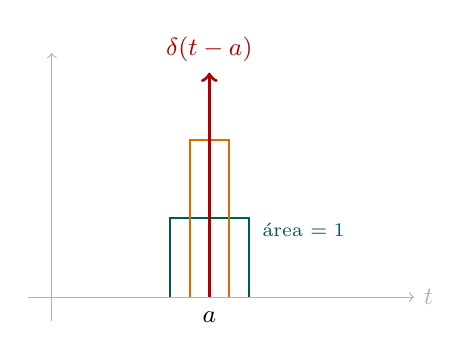
\begin{tikzpicture}[scale=1.0]
\draw[->,gray!60] (-0.3,0)--(4.6,0) node[right]{\small $t$};
\draw[->,gray!60] (0,-0.3)--(0,3.1);
% pulso ancho (area 1): ancho 1, altura 1
\draw[teal!70!black,thick] (1.5,0)--(1.5,1)--(2.5,1)--(2.5,0);
% pulso intermedio: ancho 0.5, altura 2
\draw[orange!85!black,thick] (1.75,0)--(1.75,2)--(2.25,2)--(2.25,0);
% delta simbolica
\draw[red!70!black,very thick,->] (2,0)--(2,2.85) node[above]{\small $\delta(t-a)$};
\node[below] at (2,-0.06) {\small $a$};
\node[teal!70!black,right] at (2.55,0.85) {\scriptsize área $=1$};
\end{tikzpicture}
\caption{La delta de Dirac $\delta(t-a)$ como límite de pulsos rectangulares de área $1$: al estrecharse ($\epsilon\to0^+$) la altura crece manteniendo el área, concentrando toda la masa en $t=a$ (flecha).}
\label{fig:dirac}
\end{figure}

\begin{theorem}[Transformada de la delta]
Para $a\ge0$,
\[
\mathcal{L}\{\delta(t-a)\} = e^{-as}.
\]
En particular, $\mathcal{L}\{\delta(t)\} = 1$.
\end{theorem}

\begin{example}[Respuesta impulsiva: PVI con delta]
Resolver el problema de valor inicial
\[
y'' + 4y = \delta(t-2),\qquad y(0)=0,\ y'(0)=0.
\]
\begin{myproof}
\textbf{Paso 1.} Aplicamos Laplace a ambos lados:
\[
\mathcal{L}\{y''\} + 4\mathcal{L}\{y\} = \mathcal{L}\{\delta(t-2)\}.
\]
Usando las condiciones iniciales, $\mathcal{L}\{y''\}=s^2Y(s)-s y(0)-y'(0)=s^2Y(s)$. Así,
\[
(s^2+4)Y(s) = e^{-2s}.
\]

\textbf{Paso 2.} Despejamos $Y(s)$:
\[
Y(s) = \frac{e^{-2s}}{s^2+4}.
\]

\textbf{Paso 3.} Invertimos: sabemos que $\mathcal{L}^{-1}\left\{\frac{1}{s^2+4}\right\} = \frac{1}{2}\sen(2t)$. Por el segundo teorema de traslación,
\[
y(t) = \mathcal{L}^{-1}\left\{e^{-2s}\frac{1}{s^2+4}\right\} = u(t-2)\frac{1}{2}\sen(2(t-2)).
\]
Por tanto,
\[
\boxed{y(t) = \frac{1}{2}u(t-2)\sen(2(t-2)).}
\]
\end{myproof}
\end{example}

\begin{example}[Sistema masa-resorte con impulso]
Resolver $y'' + 2y' + 5y = \delta(t-\pi)$, con $y(0)=1,\ y'(0)=0$.
\begin{myproof}
\textbf{Paso 1.} Aplicamos Laplace:
\[
\mathcal{L}\{y''\} = s^2Y - s y(0) - y'(0) = s^2Y - s,
\]
\[
\mathcal{L}\{2y'\} = 2(sY - y(0)) = 2sY - 2,
\]
\[
\mathcal{L}\{5y\} = 5Y,\qquad \mathcal{L}\{\delta(t-\pi)\}=e^{-\pi s}.
\]
La ecuación se convierte en:
\[
(s^2Y - s) + (2sY - 2) + 5Y = e^{-\pi s}.
\]

\textbf{Paso 2.} Agrupamos:
\[
(s^2+2s+5)Y - s - 2 = e^{-\pi s} \implies (s^2+2s+5)Y = s+2 + e^{-\pi s}.
\]
Luego
\[
Y(s) = \frac{s+2}{s^2+2s+5} + \frac{e^{-\pi s}}{s^2+2s+5}.
\]

\textbf{Paso 3.} Completamos cuadrado en el denominador: $s^2+2s+5 = (s+1)^2+4$.

Primera parte: $\frac{s+2}{(s+1)^2+4} = \frac{(s+1)+1}{(s+1)^2+4} = \frac{s+1}{(s+1)^2+4} + \frac{1}{2}\frac{2}{(s+1)^2+4}$.
Su inversa es: $e^{-t}\cos(2t) + \frac{1}{2}e^{-t}\sen(2t)$.

Segunda parte: $\mathcal{L}^{-1}\left\{\frac{e^{-\pi s}}{(s+1)^2+4}\right\} = u(t-\pi) \cdot \mathcal{L}^{-1}\left\{\frac{1}{(s+1)^2+4}\right\}\big|_{t\to t-\pi} = u(t-\pi)\cdot \frac{1}{2}e^{-(t-\pi)}\sen(2(t-\pi))$.

Por tanto,
\[
\boxed{y(t) = e^{-t}\cos(2t) + \frac{1}{2}e^{-t}\sen(2t) + \frac{1}{2}u(t-\pi)e^{-(t-\pi)}\sen(2(t-\pi)).}
\]
\end{myproof}
\end{example}

\section{Teorema de convolución}

\begin{definition}
La \textbf{convolución} de dos funciones $f(t)$ y $g(t)$, definidas para $t\ge0$, es la función
\[
(f * g)(t) = \int_0^t f(\tau) g(t-\tau)\,d\tau.
\]
\end{definition}

\begin{rem}
La convolución es conmutativa, asociativa y distributiva respecto a la suma. Es una operación muy útil porque permite expresar la respuesta de un sistema lineal a una entrada arbitraria en términos de su respuesta impulsiva.
\end{rem}

\begin{theorem}[Teorema de convolución]
\label{thm:cap31:convolucion}
Si $\mathcal{L}\{f(t)\}=F(s)$ y $\mathcal{L}\{g(t)\}=G(s)$, entonces
\[
\mathcal{L}\{(f * g)(t)\} = F(s) G(s).
\]
Equivalentemente,
\[
\mathcal{L}^{-1}\{F(s) G(s)\} = (f * g)(t).
\]
\end{theorem}

\begin{rem}
\emph{Esquema de la prueba.} Escribiendo el producto como integral doble,
\[
F(s)G(s)=\int_0^\infty\!\!\int_0^\infty e^{-s(\tau+\sigma)} f(\tau)g(\sigma)\,d\sigma\,d\tau,
\]
se hace el cambio $t=\tau+\sigma$ (con $\tau$ fijo, $\sigma=t-\tau$). La región $\tau,\sigma\ge0$ se convierte en $0\le\tau\le t<\infty$, y
\[
F(s)G(s)=\int_0^\infty e^{-st}\!\left(\int_0^t f(\tau)g(t-\tau)\,d\tau\right)dt=\mathcal L\{(f*g)(t)\}.
\]
\end{rem}

\begin{figure}[H]
\centering
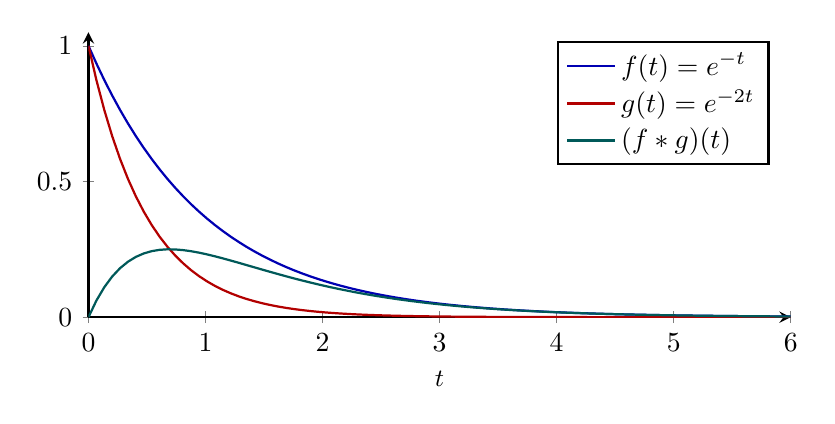
\begin{tikzpicture}
\begin{axis}[width=10.5cm,height=5.2cm,xlabel={\small $t$},domain=0:6,samples=90,
  xmin=0,xmax=6,ymin=0,ymax=1.05,axis lines=left,thick,no markers,
  legend pos=north east,legend cell align=left]
\addplot[blue!70!black]{exp(-x)};\addlegendentry{$f(t)=e^{-t}$}
\addplot[red!70!black]{exp(-2*x)};\addlegendentry{$g(t)=e^{-2t}$}
\addplot[teal!70!black,thick]{exp(-x)-exp(-2*x)};\addlegendentry{$(f*g)(t)$}
\end{axis}
\end{tikzpicture}
\caption{Convolución de $f(t)=e^{-t}$ y $g(t)=e^{-2t}$: $(f*g)(t)=\int_0^t f(\tau)g(t-\tau)\,d\tau=e^{-t}-e^{-2t}$. El Teorema~\ref{thm:cap31:convolucion} la convierte en un producto, $\mathcal L\{f*g\}=F(s)G(s)$.}
\label{fig:convolucion}
\end{figure}

\begin{example}[Inversa de un producto usando convolución]
Hallar $\mathcal{L}^{-1}\left\{\frac{1}{s^2(s^2+1)}\right\}$.
\begin{myproof}
\textbf{Paso 1.} Identificamos $F(s)=\frac{1}{s^2}$ y $G(s)=\frac{1}{s^2+1}$. Entonces
\[
f(t)=\mathcal{L}^{-1}\left\{\frac{1}{s^2}\right\}=t,\qquad g(t)=\mathcal{L}^{-1}\left\{\frac{1}{s^2+1}\right\}=\sen t.
\]

\textbf{Paso 2.} Por el teorema de convolución,
\[
\mathcal{L}^{-1}\left\{\frac{1}{s^2(s^2+1)}\right\} = (f * g)(t) = \int_0^t \tau \sen(t-\tau)\,d\tau.
\]

\textbf{Paso 3.} Calculamos la integral. Usamos la identidad $\sen(t-\tau)=\sen t\cos\tau - \cos t\sen\tau$:
\[
\int_0^t \tau (\sen t\cos\tau - \cos t\sen\tau)\,d\tau
= \sen t\int_0^t \tau\cos\tau\,d\tau - \cos t\int_0^t \tau\sen\tau\,d\tau.
\]
Integramos por partes:
\[
\int \tau\cos\tau\,d\tau = \tau\sen\tau + \cos\tau,\quad
\int \tau\sen\tau\,d\tau = -\tau\cos\tau + \sen\tau.
\]
Evaluando de $0$ a $t$:
\[
\sen t\big( t\sen t + \cos t - 1 \big) - \cos t\big( -t\cos t + \sen t \big).
\]
Simplificamos:
\[
t\sen^2 t + \sen t\cos t - \sen t + t\cos^2 t - \cos t\sen t = t(\sen^2 t+\cos^2 t) - \sen t = t - \sen t.
\]
Por tanto,
\[
\boxed{\mathcal{L}^{-1}\left\{\frac{1}{s^2(s^2+1)}\right\} = t - \sen t.}
\]
\end{myproof}
\end{example}

\begin{example}[Resolución de una EDO mediante convolución]
Resolver $y'' + y = f(t)$ con $y(0)=0,\ y'(0)=0$, donde $f(t)$ es una función arbitraria.
\begin{myproof}
\textbf{Paso 1.} Aplicamos Laplace:
\[
s^2Y(s) + Y(s) = F(s) \implies (s^2+1)Y(s)=F(s) \implies Y(s)=\frac{1}{s^2+1}F(s).
\]

\textbf{Paso 2.} Por el teorema de convolución,
\[
y(t) = \mathcal{L}^{-1}\left\{\frac{1}{s^2+1}\right\} * f(t) = \sen t * f(t) = \int_0^t \sen(t-\tau) f(\tau)\,d\tau.
\]

\textbf{Paso 3.} Esta es la solución general para cualquier entrada $f(t)$. Por ejemplo, si $f(t)=e^{t}$, entonces
\[
y(t)=\int_0^t e^{\tau}\sen(t-\tau)\,d\tau.
\]
Resolviendo la integral (o usando tabla) se obtiene $y(t)=\frac{1}{2}(e^{t}-\cos t-\sen t)$.
Por tanto,
\[
\boxed{y(t)=\int_0^t \sen(t-\tau) f(\tau)\,d\tau.}
\]
\end{myproof}
\end{example}

\begin{example}[Ecuación integral de Volterra]
Resolver $y(t) = t^2 + \int_0^t y(\tau)\sen(t-\tau)\,d\tau$.
\begin{myproof}
\textbf{Paso 1.} Observamos que la integral es la convolución $y * \sen t$. Tomamos Laplace:
\[
Y(s) = \mathcal{L}\{t^2\} + \mathcal{L}\{y * \sen t\} = \frac{2}{s^3} + Y(s)\cdot \frac{1}{s^2+1}.
\]

\textbf{Paso 2.} Despejamos $Y(s)$:
\[
Y(s)\left(1 - \frac{1}{s^2+1}\right) = \frac{2}{s^3} \implies Y(s)\left(\frac{s^2}{s^2+1}\right) = \frac{2}{s^3} \implies Y(s) = \frac{2(s^2+1)}{s^5}.
\]

\textbf{Paso 3.} Descomponemos:
\[
Y(s) = \frac{2}{s^3} + \frac{2}{s^5}.
\]
Invertimos:
\[
y(t) = 2\mathcal{L}^{-1}\left\{\frac{1}{s^3}\right\} + 2\mathcal{L}^{-1}\left\{\frac{1}{s^5}\right\}
= 2\frac{t^2}{2!} + 2\frac{t^4}{4!} = t^2 + \frac{2}{24}t^4 = t^2 + \frac{t^4}{12}.
\]
Por tanto,
\[
\boxed{y(t) = t^2 + \frac{t^4}{12}.}
\]
\end{myproof}
\end{example}

\begin{example}[Inversa de $1/(s^2+1)^2$ por convolución]
Hallar $\mathcal{L}^{-1}\left\{\dfrac{1}{(s^2+1)^2}\right\}$.
\begin{myproof}
\textbf{Paso 1.} $F(s)=G(s)=\dfrac{1}{s^2+1}$, de modo que $f=g=\sen t$.

\textbf{Paso 2.} Por el Teorema~\ref{thm:cap31:convolucion}, la inversa es la convolución $\displaystyle\int_0^t \sen\tau\,\sen(t-\tau)\,d\tau$.

\textbf{Paso 3.} Con la identidad producto-a-suma, $\dfrac{1}{2}\displaystyle\int_0^t[\cos(2\tau-t)-\cos t]\,d\tau=\dfrac{1}{2}\Big[\tfrac{\sen(2\tau-t)}{2}-\tau\cos t\Big]_0^t$.

\textbf{Paso 4.} Evaluando,
\[
\boxed{\mathcal{L}^{-1}\left\{\frac{1}{(s^2+1)^2}\right\}=\frac{\sen t-t\cos t}{2}.}
\]
\end{myproof}
\end{example}

\section{Resolución de problemas de valor inicial (PVI) con Laplace}

\begin{rem}
La estrategia general para resolver un PVI con Laplace es:
\begin{enumerate}
\item Aplicar la transformada de Laplace a ambos lados de la ecuación diferencial.
\item Usar las condiciones iniciales para expresar las transformadas de las derivadas en términos de $Y(s)$.
\item Despejar $Y(s)$.
\item Hallar $y(t)$ mediante la transformada inversa de Laplace.
\end{enumerate}
\end{rem}

\begin{example}[PVI con forzamiento continuo]
Resolver $y'' - 3y' + 2y = e^{4t}$, con $y(0)=1,\ y'(0)=0$.
\begin{myproof}
\textbf{Paso 1.} Aplicamos Laplace:
\[
\mathcal{L}\{y''\} = s^2Y - s y(0) - y'(0) = s^2Y - s,
\]
\[
\mathcal{L}\{-3y'\} = -3(sY - y(0)) = -3sY + 3,
\]
\[
\mathcal{L}\{2y\} = 2Y,\qquad \mathcal{L}\{e^{4t}\} = \frac{1}{s-4}.
\]
La ecuación se convierte en:
\[
(s^2Y - s) + (-3sY + 3) + 2Y = \frac{1}{s-4}.
\]

\textbf{Paso 2.} Agrupamos:
\[
(s^2 - 3s + 2)Y - s + 3 = \frac{1}{s-4} \implies (s-1)(s-2)Y = s - 3 + \frac{1}{s-4}.
\]
Entonces
\[
Y(s) = \frac{s-3}{(s-1)(s-2)} + \frac{1}{(s-1)(s-2)(s-4)}.
\]

\textbf{Paso 3.} Descomponemos la primera fracción: $\frac{s-3}{(s-1)(s-2)} = \frac{A}{s-1} + \frac{B}{s-2}$. $s-3 = A(s-2)+B(s-1)$. Para $s=1$: $-2 = -A \Rightarrow A=2$. Para $s=2$: $-1 = B \Rightarrow B=-1$. Luego $\frac{2}{s-1} - \frac{1}{s-2}$.

Segunda fracción: $\frac{1}{(s-1)(s-2)(s-4)} = \frac{C}{s-1} + \frac{D}{s-2} + \frac{E}{s-4}$. Multiplicando:
$1 = C(s-2)(s-4) + D(s-1)(s-4) + E(s-1)(s-2)$.
Para $s=1$: $1 = C(-1)(-3)=3C \Rightarrow C=1/3$.
Para $s=2$: $1 = D(1)(-2) = -2D \Rightarrow D=-1/2$.
Para $s=4$: $1 = E(3)(2)=6E \Rightarrow E=1/6$.

\textbf{Paso 4.} Entonces
\[
Y(s) = \frac{2}{s-1} - \frac{1}{s-2} + \frac{1/3}{s-1} - \frac{1/2}{s-2} + \frac{1/6}{s-4}
= \frac{7/3}{s-1} - \frac{3/2}{s-2} + \frac{1/6}{s-4}.
\]
Invertimos:
\[
y(t) = \frac{7}{3}e^{t} - \frac{3}{2}e^{2t} + \frac{1}{6}e^{4t}.
\]
Por tanto,
\[
\boxed{y(t) = \frac{7}{3}e^{t} - \frac{3}{2}e^{2t} + \frac{1}{6}e^{4t}.}
\]
\end{myproof}
\end{example}

\begin{example}[PVI con forzamiento discontinuo (escalón)]
Resolver $y'' + 4y = u(t-1)$, con $y(0)=0,\ y'(0)=0$.
\begin{myproof}
\textbf{Paso 1.} Aplicamos Laplace:
\[
s^2Y + 4Y = \mathcal{L}\{u(t-1)\} = \frac{e^{-s}}{s}.
\]

\textbf{Paso 2.} Despejamos:
\[
Y(s) = \frac{e^{-s}}{s(s^2+4)}.
\]

\textbf{Paso 3.} Descomponemos $\frac{1}{s(s^2+4)} = \frac{A}{s} + \frac{Bs+C}{s^2+4}$. Multiplicando:
$1 = A(s^2+4) + (Bs+C)s = A s^2 + 4A + B s^2 + C s = (A+B)s^2 + C s + 4A$.
Igualando: $A+B=0$, $C=0$, $4A=1 \Rightarrow A=1/4$, $B=-1/4$.
Luego $\frac{1}{s(s^2+4)} = \frac{1/4}{s} - \frac{1}{4}\frac{s}{s^2+4}$.

\textbf{Paso 4.} Por el segundo teorema de traslación,
\[
y(t) = u(t-1)\left[\frac{1}{4} - \frac{1}{4}\cos(2(t-1))\right].
\]
Por tanto,
\[
\boxed{y(t) = \frac{1}{4}u(t-1)\big[1 - \cos(2(t-1))\big].}
\]
\end{myproof}
\end{example}

\begin{example}[PVI con impulso (delta)]
Resolver $y'' + 2y' + 2y = \delta(t-\pi)$, con $y(0)=1,\ y'(0)=1$.
\begin{myproof}
\textbf{Paso 1.} Laplace:
\[
(s^2Y - s - 1) + 2(sY - 1) + 2Y = e^{-\pi s}.
\]
Agrupamos: $(s^2+2s+2)Y - s - 1 - 2 = e^{-\pi s} \Rightarrow (s^2+2s+2)Y = s+3 + e^{-\pi s}$.
Luego
\[
Y(s) = \frac{s+3}{(s+1)^2+1} + \frac{e^{-\pi s}}{(s+1)^2+1}.
\]

\textbf{Paso 2.} Primera parte: $\frac{s+3}{(s+1)^2+1} = \frac{(s+1)+2}{(s+1)^2+1} = \frac{s+1}{(s+1)^2+1} + 2\frac{1}{(s+1)^2+1}$.
Su inversa es: $e^{-t}\cos t + 2e^{-t}\sen t$.

\textbf{Paso 3.} Segunda parte: $\mathcal{L}^{-1}\left\{\frac{e^{-\pi s}}{(s+1)^2+1}\right\} = u(t-\pi) e^{-(t-\pi)}\sen(t-\pi)$.

\textbf{Paso 4.} Por tanto,
\[
\boxed{y(t) = e^{-t}(\cos t + 2\sen t) + u(t-\pi)e^{-(t-\pi)}\sen(t-\pi).}
\]
\end{myproof}
\end{example}

\begin{example}[PVI mixto con escalón]
Resolver $y'' + y = \begin{cases} 0, & 0\le t<2,\\ 1, & t\ge2, \end{cases}$ con $y(0)=1,\ y'(0)=0$.
\begin{myproof}
\textbf{Paso 1.} Escribimos el forzamiento como $f(t)=u(t-2)$. Aplicamos Laplace:
\[
s^2Y - s + Y = \frac{e^{-2s}}{s} \implies (s^2+1)Y = s + \frac{e^{-2s}}{s}.
\]

\textbf{Paso 2.} Despejamos:
\[
Y(s) = \frac{s}{s^2+1} + e^{-2s}\frac{1}{s(s^2+1)}.
\]

\textbf{Paso 3.} La primera inversa es $\cos t$. Para la segunda, $\frac{1}{s(s^2+1)} = \frac{1}{s} - \frac{s}{s^2+1}$ (de la descomposición anterior). Luego
\[
\mathcal{L}^{-1}\left\{e^{-2s}\left(\frac{1}{s} - \frac{s}{s^2+1}\right)\right\} = u(t-2)\big[1 - \cos(t-2)\big].
\]

\textbf{Paso 4.} Entonces
\[
\boxed{y(t) = \cos t + u(t-2)\big[1 - \cos(t-2)\big].}
\]
\end{myproof}
\end{example}

\begin{example}[PVI con forzamiento definido por tramos]
Resolver $y''+4y=\begin{cases}0,&t<1\\[2pt]2,&t\ge1\end{cases}$ con $y(0)=0$, $y'(0)=0$.
\begin{myproof}
\textbf{Paso 1.} El forzamiento es $2u(t-1)$, con $\mathcal{L}=2e^{-s}/s$. Laplace: $(s^2+4)Y=2e^{-s}/s$, luego $Y=2e^{-s}\dfrac{1}{s(s^2+4)}$.

\textbf{Paso 2.} Fracciones parciales: $\dfrac{1}{s(s^2+4)}=\dfrac{1/4}{s}-\dfrac{1}{4}\dfrac{s}{s^2+4}$.

\textbf{Paso 3.} La inversa de $\dfrac{1}{s(s^2+4)}$ es $\tfrac14(1-\cos 2t)$; el factor $e^{-s}$ activa el segundo teorema de traslación.

\textbf{Paso 4.}
\[
\boxed{y(t)=\tfrac12\, u(t-1)\big(1-\cos(2t-2)\big).}
\]
\end{myproof}
\end{example}

\section{Resolución de sistemas de EDO con Laplace}

\begin{rem}
Para un sistema de ecuaciones diferenciales lineales con coeficientes constantes, se aplica la transformada de Laplace a cada ecuación, convirtiendo el sistema diferencial en un sistema algebraico en $s$ para las transformadas de las funciones incógnita. Se resuelve el sistema algebraico y luego se invierte cada transformada.
\end{rem}

\begin{example}[Sistema homogéneo 2×2]
Resolver el sistema
\[
\begin{cases}
x' = 2x + y,\\
y' = 3x + 4y,
\end{cases}
\quad
x(0)=1,\ y(0)=0.
\]
\begin{myproof}
\textbf{Paso 1.} Aplicamos Laplace. Sea $X=\mathcal{L}\{x\}$, $Y=\mathcal{L}\{y\}$.
\[
sX - x(0) = 2X + Y \implies (s-2)X - Y = 1.
\]
\[
sY - y(0) = 3X + 4Y \implies -3X + (s-4)Y = 0.
\]

\textbf{Paso 2.} Resolvemos el sistema algebraico. De la segunda, $Y = \frac{3}{s-4}X$. Sustituimos en la primera:
\[
(s-2)X - \frac{3}{s-4}X = 1 \implies X\left( s-2 - \frac{3}{s-4} \right) = 1 \implies X \frac{(s-2)(s-4)-3}{s-4} = 1.
\]
$(s-2)(s-4)-3 = s^2-6s+8-3 = s^2-6s+5 = (s-1)(s-5)$.
Así,
\[
X = \frac{s-4}{(s-1)(s-5)},\qquad Y = \frac{3}{s-4}X = \frac{3}{(s-1)(s-5)}.
\]

\textbf{Paso 3.} Descomponemos $X$:
\[
\frac{s-4}{(s-1)(s-5)} = \frac{A}{s-1} + \frac{B}{s-5}.
\]
$s-4 = A(s-5)+B(s-1)$. Para $s=1$: $-3 = A(-4) \Rightarrow A=3/4$. Para $s=5$: $1 = B(4) \Rightarrow B=1/4$.
Entonces $X = \frac{3/4}{s-1} + \frac{1/4}{s-5}$.

Para $Y$: $\frac{3}{(s-1)(s-5)} = \frac{C}{s-1} + \frac{D}{s-5}$.
$3 = C(s-5)+D(s-1)$. Para $s=1$: $3 = C(-4) \Rightarrow C=-3/4$. Para $s=5$: $3 = D(4) \Rightarrow D=3/4$.
Entonces $Y = \frac{-3/4}{s-1} + \frac{3/4}{s-5}$.

\textbf{Paso 4.} Invertimos:
\[
x(t) = \frac{3}{4}e^{t} + \frac{1}{4}e^{5t},\qquad y(t) = -\frac{3}{4}e^{t} + \frac{3}{4}e^{5t}.
\]
Por tanto,
\[
\boxed{x(t) = \frac{3}{4}e^{t} + \frac{1}{4}e^{5t},\qquad y(t) = -\frac{3}{4}e^{t} + \frac{3}{4}e^{5t}.}
\]
\end{myproof}
\end{example}

\begin{example}[Sistema no homogéneo]
Resolver
\[
\begin{cases}
x' + x - y = 2t,\\
y' + x + y = 0,
\end{cases}
\quad
x(0)=0,\ y(0)=1.
\]
\begin{myproof}
\textbf{Paso 1.} Aplicamos Laplace:
\[
(sX - x(0)) + X - Y = \frac{2}{s^2} \implies (s+1)X - Y = \frac{2}{s^2}.
\]
\[
(sY - y(0)) + X + Y = 0 \implies X + (s+1)Y = 1.
\]

\textbf{Paso 2.} Resolvemos. Despejamos $Y = (s+1)X - \frac{2}{s^2}$ de la primera. Sustituimos en la segunda:
\[
X + (s+1)\left((s+1)X - \frac{2}{s^2}\right) = 1 \implies X\big(1+(s+1)^2\big) - \frac{2(s+1)}{s^2} = 1.
\]
\[
X = \frac{1 + \frac{2(s+1)}{s^2}}{1+(s+1)^2} = \frac{s^2 + 2s + 2}{s^2(s^2+2s+2)}.
\]
Observamos que $s^2+2s+2$ se cancela con el numerador (pues $s^2+2s+2$ es el mismo). Así,
\[
X = \frac{1}{s^2}.
\]
Luego $Y = (s+1)X - \frac{2}{s^2} = \frac{s+1}{s^2} - \frac{2}{s^2} = \frac{s-1}{s^2} = \frac{1}{s} - \frac{1}{s^2}$.

\textbf{Paso 3.} Invertimos:
\[
x(t) = \mathcal{L}^{-1}\left\{\frac{1}{s^2}\right\} = t,
\]
\[
y(t) = \mathcal{L}^{-1}\left\{\frac{1}{s} - \frac{1}{s^2}\right\} = 1 - t.
\]

\textbf{Paso 4.} Comprobamos las condiciones iniciales: $x(0)=0$, $y(0)=1$. Por tanto,
\[
\boxed{x(t)=t,\qquad y(t)=1-t.}
\]
\end{myproof}
\end{example}

\begin{example}[Sistema $2\times2$ resuelto con Laplace]
Resolver $x'=x+y$, $y'=4x+y$ con $x(0)=1$, $y(0)=0$.
\begin{myproof}
\textbf{Paso 1.} Transformando: $(s-1)X-Y=1$ y $-4X+(s-1)Y=0$.

\textbf{Paso 2.} De la segunda, $Y=\dfrac{4}{s-1}X$; sustituyendo, $X\dfrac{(s-1)^2-4}{s-1}=1$, luego
\[
X=\frac{s-1}{(s-3)(s+1)},\qquad Y=\frac{4}{(s-3)(s+1)}.
\]

\textbf{Paso 3.} Fracciones parciales: $X=\dfrac{1/2}{s-3}+\dfrac{1/2}{s+1}$, $\;Y=\dfrac{1}{s-3}-\dfrac{1}{s+1}$.

\textbf{Paso 4.} Invirtiendo,
\[
\boxed{x(t)=\tfrac12(e^{3t}+e^{-t}),\qquad y(t)=e^{3t}-e^{-t}.}
\]
\end{myproof}
\end{example}

\section{Aplicaciones}

\subsection{Circuitos RLC con interruptor}

\begin{rem}
La ecuación que rige la carga $Q(t)$ en un circuito RLC en serie es
\[
L Q'' + R Q' + \frac{1}{C}Q = E(t),
\]
donde $E(t)$ es la fuerza electromotriz (voltaje aplicado). Si se conecta una fuente de voltaje constante $E_0$ en el instante $t=a$, entonces $E(t)=E_0 u(t-a)$.
\end{rem}

\begin{example}[Circuito RLC con conexión escalón]
Un circuito RLC tiene $L=1$ H, $R=3$ $\Omega$, $C=1/2$ F. En $t=2$ s se conecta una fuente de $10$ V. Hallar $Q(t)$ si inicialmente $Q(0)=0,\ I(0)=Q'(0)=0$.
\begin{myproof}
\textbf{Paso 1.} La ecuación es $Q'' + 3Q' + 2Q = 10 u(t-2)$ (pues $1/C = 2$). Aplicamos Laplace:
\[
s^2Q(s) + 3sQ(s) + 2Q(s) = \frac{10 e^{-2s}}{s}.
\]

\textbf{Paso 2.} Despejamos:
\[
Q(s) = \frac{10 e^{-2s}}{s(s^2+3s+2)} = 10 e^{-2s}\frac{1}{s(s+1)(s+2)}.
\]

\textbf{Paso 3.} Descomponemos $\frac{1}{s(s+1)(s+2)} = \frac{A}{s} + \frac{B}{s+1} + \frac{C}{s+2}$.
$1 = A(s+1)(s+2) + B s(s+2) + C s(s+1)$.
Para $s=0$: $1 = A(1)(2)=2A \Rightarrow A=1/2$.
Para $s=-1$: $1 = B(-1)(1) = -B \Rightarrow B=-1$.
Para $s=-2$: $1 = C(-2)(-1)=2C \Rightarrow C=1/2$.
Luego $\frac{1}{s(s+1)(s+2)} = \frac{1/2}{s} - \frac{1}{s+1} + \frac{1/2}{s+2}$.

\textbf{Paso 4.} Por el segundo teorema de traslación:
\[
Q(t) = 10 u(t-2)\left[ \frac{1}{2} - e^{-(t-2)} + \frac{1}{2}e^{-2(t-2)} \right].
\]
Por tanto,
\[
\boxed{Q(t) = 5u(t-2)\left(1 - 2e^{-(t-2)} + e^{-2(t-2)}\right).}
\]
\end{myproof}
\end{example}

\subsection{Sistemas mecánicos con forzamiento discontinuo}

\begin{rem}
Para un sistema masa-resorte-amortiguador, la ecuación es $m y'' + c y' + k y = F(t)$, donde $F(t)$ es la fuerza externa. Si la fuerza se activa en $t=a$, entonces $F(t)=F_0 u(t-a)$.
\end{rem}

\begin{example}[Respuesta a una fuerza escalón]
Resolver $y'' + 4y' + 4y = 3u(t-1)$, con $y(0)=0,\ y'(0)=0$. Interpretar físicamente.
\begin{myproof}
\textbf{Paso 1.} Aplicamos Laplace:
\[
(s^2+4s+4)Y = \frac{3e^{-s}}{s} \implies Y = \frac{3e^{-s}}{s(s+2)^2}.
\]

\textbf{Paso 2.} Descomponemos $\frac{1}{s(s+2)^2} = \frac{A}{s} + \frac{B}{s+2} + \frac{C}{(s+2)^2}$.
$1 = A(s+2)^2 + B s(s+2) + C s$.
Para $s=0$: $1 = 4A \Rightarrow A=1/4$.
Para $s=-2$: $1 = C(-2) \Rightarrow C=-1/2$.
Para $s=1$ (por ejemplo): $1 = A(9) + B(3) + C(1) = 9/4 + 3B - 1/2 = 7/4 + 3B \Rightarrow 3B = -3/4 \Rightarrow B=-1/4$.
Así, $\frac{1}{s(s+2)^2} = \frac{1/4}{s} - \frac{1/4}{s+2} - \frac{1/2}{(s+2)^2}$.

\textbf{Paso 3.} Multiplicamos por $3e^{-s}$:
\[
Y = 3e^{-s}\left( \frac{1/4}{s} - \frac{1/4}{s+2} - \frac{1/2}{(s+2)^2} \right).
\]

\textbf{Paso 4.} Invertimos:
\[
y(t) = 3u(t-1)\left[ \frac{1}{4} - \frac{1}{4}e^{-2(t-1)} - \frac{1}{2}(t-1)e^{-2(t-1)} \right].
\]
Por tanto,
\[
\boxed{y(t) = \frac{3}{4}u(t-1)\left( 1 - e^{-2(t-1)} - 2(t-1)e^{-2(t-1)} \right).}
\]
La posición y la velocidad son continuas en $t=1$; la aceleración presenta una discontinuidad debido a la fuerza escalón.
\end{myproof}
\end{example}

\subsection{Respuesta impulsiva y función de Green}

\begin{rem}
La respuesta al impulso unitario (función de Green) es la solución de $m y'' + c y' + k y = \delta(t-a)$ con condiciones iniciales nulas. Su transformada es
\[
Y(s) = \frac{e^{-as}}{m s^2 + c s + k} = e^{-as} H(s),
\]
donde $H(s)$ es la función de transferencia. La respuesta impulsiva es $h(t-a)$ con $h(t)=\mathcal{L}^{-1}\{H(s)\}$.
\end{rem}

\begin{example}[Función de Green para un sistema críticamente amortiguado]
Hallar la respuesta impulsiva de $y'' + 4y' + 4y = \delta(t)$ con $y(0)=0,\ y'(0)=0$.
\begin{myproof}
\textbf{Paso 1.} Aplicamos Laplace: $(s^2+4s+4)Y = 1 \implies Y(s)=\frac{1}{(s+2)^2}$.

\textbf{Paso 2.} Invertimos: $\mathcal{L}^{-1}\left\{\frac{1}{(s+2)^2}\right\} = t e^{-2t}$.

\textbf{Paso 3.} Esta es la respuesta a un impulso en $t=0$. Para un impulso en $t=a$, sería $(t-a)e^{-2(t-a)}u(t-a)$.
Por tanto,
\[
\boxed{h(t) = t e^{-2t}.}
\]
\end{myproof}
\end{example}

\section{Problemas resueltos adicionales}

% Básico
\begin{prob}[Cálculo directo]
Calcular $\mathcal{L}\{5t^3 - 2\sen(4t) + e^{3t}\}$.
\begin{myproof}
\textbf{Paso 1.} Usamos linealidad y la tabla:
\[
\mathcal{L}\{5t^3\} = 5\frac{3!}{s^4}=\frac{30}{s^4},\quad
\mathcal{L}\{-2\sen(4t)\} = -2\frac{4}{s^2+16} = -\frac{8}{s^2+16},\quad
\mathcal{L}\{e^{3t}\}=\frac{1}{s-3}.
\]
\textbf{Paso 2.} Sumamos:
\[
\boxed{\frac{30}{s^4} - \frac{8}{s^2+16} + \frac{1}{s-3}.}
\]
\end{myproof}
\end{prob}

% Básico
\begin{prob}[Primer teorema de traslación]
Hallar $\mathcal{L}\{e^{-t}\cos(2t)\}$.
\begin{myproof}
\textbf{Paso 1.} $f(t)=\cos(2t)$, $F(s)=\frac{s}{s^2+4}$. Con $a=-1$, $F(s+1)=\frac{s+1}{(s+1)^2+4}$.
\[
\boxed{\frac{s+1}{(s+1)^2+4}.}
\]
\end{myproof}
\end{prob}

% Intermedio
\begin{prob}[Transformada de derivada]
Si $\mathcal{L}\{y\}=Y$, y $y(0)=2,\ y'(0)=-1$, calcular $\mathcal{L}\{y''-3y'\}$ en términos de $Y$.
\begin{myproof}
\textbf{Paso 1.} $\mathcal{L}\{y''\}=s^2Y - s(2) - (-1)=s^2Y -2s+1$.
\textbf{Paso 2.} $\mathcal{L}\{-3y'\} = -3(sY - 2) = -3sY+6$.
\textbf{Paso 3.} Sumamos: $(s^2-3s)Y -2s+7$.
\[
\boxed{(s^2-3s)Y -2s + 7.}
\]
\end{myproof}
\end{prob}

% Intermedio
\begin{prob}[Multiplicación por $t$]
Calcular $\mathcal{L}\{t\cos(3t)\}$.
\begin{myproof}
\textbf{Paso 1.} $F(s)=\frac{s}{s^2+9}$. $F'(s)=\frac{9-s^2}{(s^2+9)^2}$.
\textbf{Paso 2.} $\mathcal{L}\{t\cos(3t)\} = -F'(s) = \frac{s^2-9}{(s^2+9)^2}$.
\[
\boxed{\frac{s^2-9}{(s^2+9)^2}.}
\]
\end{myproof}
\end{prob}

% Desafiante
\begin{prob}[División por $t$]
Calcular $\mathcal{L}\left\{\frac{1-\cos t}{t}\right\}$.
\begin{myproof}
\textbf{Paso 1.} $f(t)=1-\cos t$, $F(s)=\frac{1}{s} - \frac{s}{s^2+1}$.
\textbf{Paso 2.} $\int_s^\infty \left(\frac{1}{u} - \frac{u}{u^2+1}\right) du = [\ln u - \frac{1}{2}\ln(u^2+1)]_s^\infty = \lim_{u\to\infty}\ln\frac{u}{\sqrt{u^2+1}} - \ln\frac{s}{\sqrt{s^2+1}}$.
\textbf{Paso 3.} El límite es $\ln 1 = 0$. Resultado: $\ln\frac{\sqrt{s^2+1}}{s} = \frac{1}{2}\ln\frac{s^2+1}{s^2}$.
\[
\boxed{\frac{1}{2}\ln\left(1+\frac{1}{s^2}\right).}
\]
\end{myproof}
\end{prob}

% Básico
\begin{prob}[Fracciones parciales raíces reales]
Hallar $\mathcal{L}^{-1}\left\{\frac{2s+1}{s^2-5s+6}\right\}$.
\begin{myproof}
\textbf{Paso 1.} Factor: $(s-2)(s-3)$. Descomponer: $\frac{A}{s-2}+\frac{B}{s-3}$.
$2s+1 = A(s-3)+B(s-2)$. $s=2$: $5=-A\Rightarrow A=-5$. $s=3$: $7=B$.
\textbf{Paso 2.} Inversa: $-5e^{2t}+7e^{3t}$.
\[
\boxed{-5e^{2t}+7e^{3t}.}
\]
\end{myproof}
\end{prob}

% Básico
\begin{prob}[Raíces repetidas]
Hallar $\mathcal{L}^{-1}\left\{\frac{s}{(s-1)^2}\right\}$.
\begin{myproof}
\textbf{Paso 1.} Escribir $\frac{s}{(s-1)^2} = \frac{(s-1)+1}{(s-1)^2} = \frac{1}{s-1} + \frac{1}{(s-1)^2}$.
\textbf{Paso 2.} Inversa: $e^t + t e^t$.
\[
\boxed{e^t(1+t).}
\]
\end{myproof}
\end{prob}

% Intermedio
\begin{prob}[Completación de cuadrados]
Hallar $\mathcal{L}^{-1}\left\{\frac{2s+5}{s^2+6s+13}\right\}$.
\begin{myproof}
\textbf{Paso 1.} $(s+3)^2+4$. Numerador: $2s+5 = 2(s+3)-1$.
\textbf{Paso 2.} $=2\frac{s+3}{(s+3)^2+4} - \frac{1}{2}\frac{2}{(s+3)^2+4}$.
\textbf{Paso 3.} Inversa: $2e^{-3t}\cos(2t) - \frac{1}{2}e^{-3t}\sen(2t)$.
\[
\boxed{e^{-3t}\left(2\cos 2t - \frac{1}{2}\sen 2t\right).}
\]
\end{myproof}
\end{prob}

% Básico
\begin{prob}[Segundo teorema de traslación directo]
Calcular $\mathcal{L}\{u(t-4)(t-4)^2\}$.
\begin{myproof}
\textbf{Paso 1.} $f(t)=t^2$, $F(s)=2/s^3$. $a=4$.
\textbf{Paso 2.} $e^{-4s}\frac{2}{s^3}$.
\[
\boxed{\frac{2e^{-4s}}{s^3}.}
\]
\end{myproof}
\end{prob}

% Intermedio
\begin{prob}[Inversa con escalón]
Hallar $\mathcal{L}^{-1}\left\{\frac{e^{-2s}}{s^2+9}\right\}$.
\begin{myproof}
\textbf{Paso 1.} $F(s)=\frac{1}{s^2+9}$, $f(t)=\frac{1}{3}\sen(3t)$.
\textbf{Paso 2.} Por traslación: $u(t-2)\frac{1}{3}\sen(3(t-2))$.
\[
\boxed{\frac{1}{3}u(t-2)\sen(3t-6).}
\]
\end{myproof}
\end{prob}

% Intermedio
\begin{prob}[Transformada de escalón general]
Calcular $\mathcal{L}\{u(t-\pi)\cos t\}$.
\begin{myproof}
\textbf{Paso 1.} Usar forma alternativa: $e^{-\pi s}\mathcal{L}\{\cos(t+\pi)\} = e^{-\pi s}\mathcal{L}\{-\cos t\}$.
\textbf{Paso 2.} $= -e^{-\pi s}\frac{s}{s^2+1}$.
\[
\boxed{-\frac{s e^{-\pi s}}{s^2+1}.}
\]
\end{myproof}
\end{prob}

% Básico
\begin{prob}[Delta de Dirac directa]
Calcular $\mathcal{L}\{\delta(t-5)\}$.
\begin{myproof}
\textbf{Paso 1.} Por definición, $\mathcal{L}\{\delta(t-a)\}=e^{-as}$.
\textbf{Paso 2.} Con $a=5$, $\boxed{e^{-5s}}$.
\end{myproof}
\end{prob}

% Intermedio
\begin{prob}[PVI continuo]
Resolver $y'' - 2y' - 3y = 0$, $y(0)=1,\ y'(0)=2$.
\begin{myproof}
\textbf{Paso 1.} $(s^2-2s-3)Y - s + 2 - 2 = 0 \Rightarrow (s-3)(s+1)Y = s$.
\textbf{Paso 2.} $Y=\frac{s}{(s-3)(s+1)} = \frac{A}{s-3}+\frac{B}{s+1}$. $s = A(s+1)+B(s-3)$. $s=3$: $3=4A\Rightarrow A=3/4$. $s=-1$: $-1=-4B\Rightarrow B=1/4$.
\textbf{Paso 3.} $y(t)=\frac{3}{4}e^{3t} + \frac{1}{4}e^{-t}$.
\[
\boxed{\frac{3}{4}e^{3t}+\frac{1}{4}e^{-t}.}
\]
\end{myproof}
\end{prob}

% Intermedio
\begin{prob}[PVI con escalón]
Resolver $y' + 2y = u(t-1)$, $y(0)=0$.
\begin{myproof}
\textbf{Paso 1.} $sY + 2Y = e^{-s}/s \Rightarrow Y = e^{-s}\frac{1}{s(s+2)}$.
\textbf{Paso 2.} $\frac{1}{s(s+2)} = \frac{1/2}{s} - \frac{1/2}{s+2}$.
\textbf{Paso 3.} $y(t)=\frac{1}{2}u(t-1)(1 - e^{-2(t-1)})$.
\[
\boxed{\frac{1}{2}u(t-1)(1-e^{-2(t-1)}).}
\]
\end{myproof}
\end{prob}

% Intermedio
\begin{prob}[PVI con delta]
Resolver $y'' + y = \delta(t-\pi/2)$, $y(0)=0,\ y'(0)=1$.
\begin{myproof}
\textbf{Paso 1.} $(s^2+1)Y - 1 = e^{-\pi s/2} \Rightarrow Y = \frac{1}{s^2+1} + \frac{e^{-\pi s/2}}{s^2+1}$.
\textbf{Paso 2.} Inversa: $\sen t + u(t-\pi/2)\sen(t-\pi/2)$.
\textbf{Paso 3.} $\sen(t-\pi/2)=-\cos t$. Entonces $y(t)=\sen t - u(t-\pi/2)\cos t$.
\[
\boxed{\sen t - u(t-\pi/2)\cos t.}
\]
\end{myproof}
\end{prob}

% Intermedio
\begin{prob}[Sistema no homogéneo 2×2]
Resolver $x' = -x + y$, $y' = x - y$, con $x(0)=0,\ y(0)=1$.
\begin{myproof}
\textbf{Paso 1.} $sX + X - Y = 0 \Rightarrow (s+1)X - Y = 0$. $-X + (s+1)Y = 1$.
\textbf{Paso 2.} De la primera, $Y=(s+1)X$. Sustituir: $-X + (s+1)^2 X = 1 \Rightarrow X((s+1)^2-1)=1 \Rightarrow X(s^2+2s)=1 \Rightarrow X = \frac{1}{s(s+2)}$.
$Y = (s+1)X = \frac{s+1}{s(s+2)}$.
\textbf{Paso 3.} Descomponer $X = \frac{1/2}{s} - \frac{1/2}{s+2}$. $Y = \frac{s+1}{s(s+2)} = \frac{A}{s}+\frac{B}{s+2}$. $s+1 = A(s+2)+B s$. $s=0$: $1=2A\Rightarrow A=1/2$. $s=-2$: $-1=-2B\Rightarrow B=1/2$. $Y = \frac{1/2}{s}+\frac{1/2}{s+2}$.
\textbf{Paso 4.} $x(t)=\frac{1}{2} - \frac{1}{2}e^{-2t}$, $y(t)=\frac{1}{2}+\frac{1}{2}e^{-2t}$.
\[
\boxed{x(t)=\frac{1}{2}(1-e^{-2t}),\quad y(t)=\frac{1}{2}(1+e^{-2t}).}
\]
\end{myproof}
\end{prob}

% Desafiante
\begin{prob}[Aplicación: circuito RLC]
Un circuito RLC con $L=1$ H, $R=2$ $\Omega$, $C=1$ F tiene aplicado un voltaje $E(t)=5u(t-3)$ V. Si $Q(0)=0,\ I(0)=0$, hallar $Q(t)$.
\begin{myproof}
\textbf{Paso 1.} $Q'' + 2Q' + Q = 5u(t-3)$. Laplace: $(s^2+2s+1)Y = 5e^{-3s}/s \Rightarrow Y = 5e^{-3s}\frac{1}{s(s+1)^2}$.
\textbf{Paso 2.} $\frac{1}{s(s+1)^2} = \frac{1}{s} - \frac{1}{s+1} - \frac{1}{(s+1)^2}$ (descomposición: $A=1, B=-1, C=-1$).
\textbf{Paso 3.} $Q(t)=5u(t-3)[1 - e^{-(t-3)} - (t-3)e^{-(t-3)}]$.
\[
\boxed{5u(t-3)\left(1 - e^{-(t-3)} - (t-3)e^{-(t-3)}\right).}
\]
\end{myproof}
\end{prob}

% Desafiante
\begin{prob}[Aplicación: masa-resorte con impulso]
Un sistema masa-resorte no amortiguado ($m=1,\ k=4$) recibe un golpe en $t=2$ que aplica una fuerza $\delta(t-2)$. Si parte del reposo, hallar la posición $y(t)$.
\begin{myproof}
\textbf{Paso 1.} $y'' + 4y = \delta(t-2)$, $y(0)=0,\ y'(0)=0$.
\textbf{Paso 2.} $(s^2+4)Y = e^{-2s} \Rightarrow Y = e^{-2s}\frac{1}{s^2+4}$.
\textbf{Paso 3.} Inversa: $y(t)=u(t-2)\frac{1}{2}\sen(2(t-2))$.
\[
\boxed{\frac{1}{2}u(t-2)\sen(2t-4).}
\]
\end{myproof}
\end{prob}

\section{Problemas propuestos}

% Básico
\begin{prob}
Calcule $\mathcal{L}\{3t^2 - e^{-2t} + \sen 5t\}$.
\end{prob}

\begin{prob}
Calcule $\mathcal{L}\{e^{2t}\sen 3t\}$ (primer teorema de traslación).
\end{prob}

\begin{prob}
Halle $\mathcal{L}^{-1}\left\{\dfrac{s+2}{s^2+4}\right\}$.
\end{prob}

\begin{prob}
Calcule $\mathcal{L}\{\delta(t-2)+u(t-3)\}$.
\end{prob}

\begin{prob}
Halle $\mathcal{L}^{-1}\left\{\dfrac{1}{(s-1)(s+2)}\right\}$ por fracciones parciales.
\end{prob}

% Intermedio
\begin{prob}
Halle $\mathcal{L}^{-1}\left\{\dfrac{s}{s^2+4s+13}\right\}$ (completación de cuadrados).
\end{prob}

\begin{prob}
Calcule $\mathcal{L}\{u(t-2)(t-2)^3\}$ (segundo teorema de traslación).
\end{prob}

\begin{prob}
Calcule $\mathcal{L}\{t^2 e^{-t}\}$.
\end{prob}

\begin{prob}
Resuelva el PVI $y'' - 3y' + 2y = e^{3t}$ con $y(0)=0$, $y'(0)=0$.
\end{prob}

\begin{prob}
Resuelva el PVI $y' + 3y = u(t-2)$ con $y(0)=1$.
\end{prob}

\begin{prob}
Resuelva el PVI $y'' + 2y' + y = \delta(t-1)$ con $y(0)=0$, $y'(0)=0$.
\end{prob}

\begin{prob}
Halle $\mathcal{L}^{-1}\left\{\dfrac{1}{s(s^2+4)}\right\}$ (por convolución o fracciones parciales).
\end{prob}

% Desafiante
\begin{prob}
Resuelva con Laplace el sistema $x'=2x-y$, $y'=x+2y$, con $x(0)=1$, $y(0)=0$.
\end{prob}

\begin{prob}
Resuelva $y'' + 2y' + 2y = \delta(t) + u(t-\pi)$ con $y(0)=0$, $y'(0)=0$.
\end{prob}

\begin{prob}
Un circuito RL con $L=1$ H, $R=3\ \Omega$ recibe $E(t)=10\,u(t-1)-10\,u(t-2)$ V. Halle $i(t)$ con $i(0)=0$.
\end{prob}
